\chapter{Introduction}
%St : 1 

%Increasing resolution -> motivation and difficulties st 1
Throughout the history of astronomy, there have been celestial sources which appear point-like (unresolved) with the available instrumentation. To clarify the nature of these sources, ever more sophisticated instruments are developed. 

In principle, a diffraction-limited aperture can obtain an angular resolution of
\begin{equation}\label{eq:ang_res}
 \theta_{\rm res}\ \approx \ 1.22\ \lambda / D,
\end{equation}
where $D$ is the diameter of the aperture and $\lambda$ is the observing wavelength. However, dish apertures larger than a hundred metres are infeasible to construct while systematic errors, including scattering-induced blurring due to turbulence in the Earth's atmosphere can lead to instrument being unable to reach the diffraction limit. To overcome these difficulties and improve $\theta_{\rm res}$, a variety of new technologies have been developed, including space-based observatories which bypass the Earth's atmosphere, interferometric arrays which eliminate the need to build extremely large apertures, as well as mitigation strategies like adaptive optics and water vapour radiometry which account for atmospheric turbulence in real time.  


%Very Long Baseline Interferometry -> the highest resolution st 1
The astronomical observatory which typically achieves the highest angular resolution is Very Long Baseline Interferometry (VLBI). Interferometry  refers to the technique of measuring the electric field correlations (named `visibilities') between pairs of separated antennae. The visibilities can be related to Fourier components on a section of approximately flat sky. Through an `adequate' sampling of the Fourier domain an approximate image of sky can be reconstructed using the inverse Fourier transform. With this method, the distance between the antennae ($\bm{b}$, referred to as the `baseline') effectively replaces $D$ in equation~\ref{eq:ang_res}, yielding a much finer angular resolution than a single aperture. This technique is primarily used at radio frequencies as the phase of the electric field becomes unstable at shorter wavelengths, which causes the averaging during correlation to become incoherent. Hence, VLBI is simply radio interferometry with antennae separated by large distances, typically $\gtrsim 100$~km, including the possibility for antennae in Earth's orbit. The technique has seen several noteworthy achievements since its inception in the late 1960's, including resolution of the extra-galactic, compact, highly-variable objects, now known as quasars into super-luminal core-jet systems \citep[e.g.][]{Whitney_1971}, and the mapping of maser motion around the Super-Massive Black Holes (SMBH) in the cores of nearby galaxies \citep[e.g.][]{Miyoshi_1995}.

\section{The Event Horizon Telescope (EHT)}
% St: 1

% EHT -> intro to the Array st 1
In the last few decades there has been a push to enable VLBI capabilities at sub-millimetre wavelengths. This effort is being led by the Event Horizon Telescope consortium \citep[(EHT),][]{Doeleman_2010}, an international project whose primary objective is to spatially resolve nearby SMBHs with an angular resolution on the order of their event horizons. In contrast to competing high frequency VLBI observatories e.g. the Very Long Baseline Array (VLBA) and the European VLBI network (EVN) which have coverage to 87~GHz (3~mm), the EHT is currently observing at 230~GHz (1.3~mm) and will potentially extend till 315~GHz (0.8~mm) in the future. See Fig.~\ref{fig:eht_globe} for an annotated map of the locations of the EHT array. As the EHT will have baseline lengths comparable to the diameter of the earth, $|b| \sim 10^4$~km and is currently observing at 1.3~mm, this yields $\theta_{\rm res} \sim 30\ \mu$-arcsec.

%st 1
\begin{figure}
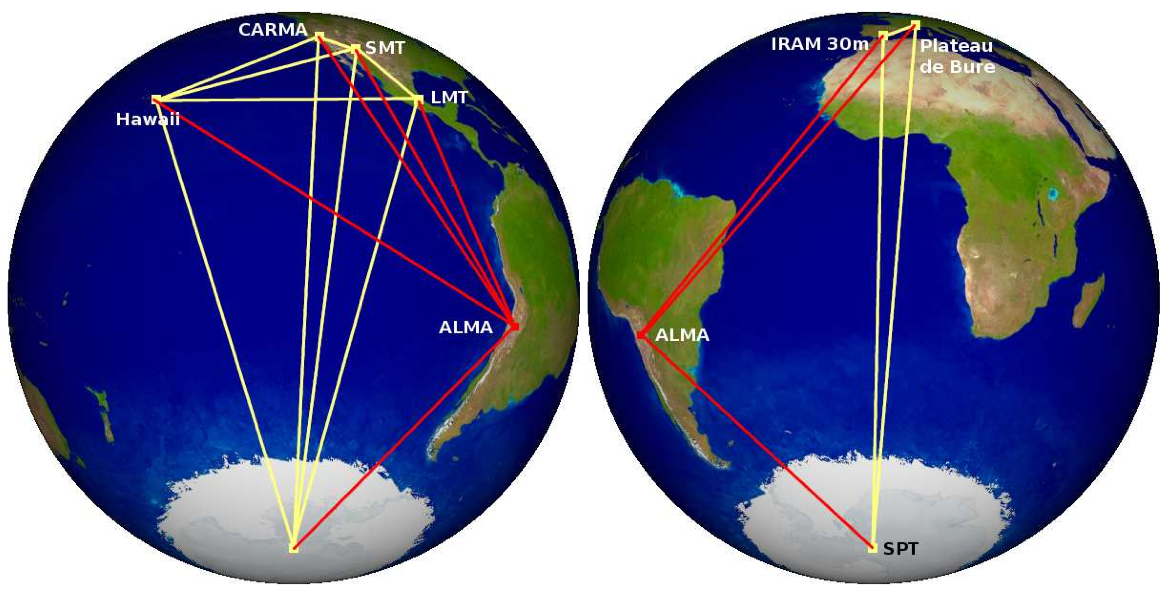
\includegraphics[width=0.8\columnwidth]{Images/eht_globe}
\caption{(Image credit: Remo Tilanius) The view of the Event Horizon Telescope (EHT) from Sgr~A*. This interferometric array uses Earth-diameter baselines, operating at $230-315$~GHz to attain resolution on order of ${\theta_{\rm res} \sim 10\ \mu}$-arcsec. Baselines to ALMA are shown in red, highlighting it's order of magnitude higher sensitivity. Note that the CARMA station has recently been discontinued, a telescope in Greenland is currently being constructed and there is ongoing investigation into a possible site in Southern Africa.\label{fig:eht_globe}%
}
\end{figure}

% EHT -> intro to the science : scales st 1
To constrain the physics near a black hole, the observation needs to be sensitive to scales comparable to the event horizon. For a non-spinning (Schwarschild) black hole, the event horizon is spherically symmetric with a radius, 
\begin{equation}
R_{\rm Sch} = 2 G M_{\rm BH} /c^2,
\end{equation}
where $M_{\rm BH}$ is the black hole mass, $G$ is the gravitational constant and $c$ is the speed of light. The angular size of such an event horizon in the far field approximation is
\begin{align}
\theta_{\rm Sch} &= R_{\rm Sch} / d_{\rm src}\\
&\approx 0.02^{\prime \prime} \times 10^{-9} (M_{\rm BH}/M_\odot)({\rm kpc}/d_{\rm src}),
\end{align}
where $d_{\rm src}$ is the distance from observer to source. For Sgr~A$^\star$, optical monitoring of stars orbiting Sgr~A* \citep{Gillessen_2009} has yielded ${M_{\rm BH} = 4.30 \pm 0.36 \times 10^{6} M_\odot}$ and ${d_{\rm src}= 8.28 \pm 0.32}$~kpc which results in ${\theta_{\rm Sch} \approx 10\ \mu}$-arcsec. 

%Lensing and the photon ring  st 1
Fortunately, the innermost emission is gravitationally lensed by the SMBH, which causes it to appear magnified by several times its original size. In theory, the innermost orbit should be dominated by a ring of photons, the lensed image of which should feature a shadow-like (or `silhouette') feature \citep[e.g.][]{Johannsen_2010}. Fig.~\ref{fig:grmhd} shows an image ray-traced from a General Relativistic Magneto-Hydrodynamic simulation of the accretion disc around Sgr~A* \citep{Moscibrodzka_2014} The circular shadow is apparent in the centre of the image. The two primary targets Sgr~A$^\star$ and M87 are expected to have gravitationally-lensed photon rings with apparent angular diameters of $\theta_{\rm pr} \sim 50$ and $\sim 20-40\ \mu$-arcsec respectively \citep*{Broderick_2009,Falcke_2013}, and hence should be resolvable by the EHT. 

% Emission and optical depth st 1
There are other important reasons why this observation needs to be conducted near sub-millimetre frequencies. Firstly, the power spectrum of Sgr~A$^\star$ peaks sharply in sub-millimetre, which for a self-absorbed synchrotron source  implies that the emission becomes optically thin and at these frequencies, that the emission arises from event horizon scales \citep{Serabyn_1997,Falcke_1998}. Hence observations at the sub-millimetre are sensitive to the innermost emission.
%ISM blurring st 1
The second reason is that blurring effects, induced by scattering in the Interstellar Medium (ISM) in the direction of the Galactic Centre \citep[e.g.][]{Fish_2014} fall as $\nu^{-2}$ and become subdominant to intrinsic structure in the sub-millimetre range.


%st 1
\begin{figure}
\begin{center}
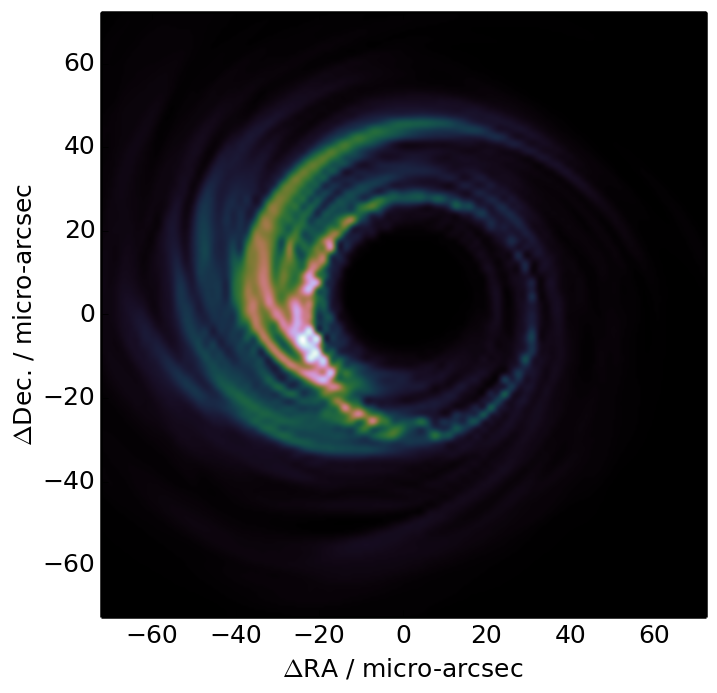
\includegraphics[width=0.5\columnwidth]{Images/disk30}
\caption{GR-MHD simulation of an accretion disk inclined at $30^\circ$ around Sgr~A* from \citet{Moscibrodzka_2014}. The dark area in the centre, known as the black hole shadow is the lensed image of the photon ring orbiting the BH. A measurement of it's precise shape is a test of general relativity in the strong field regime. Note that the left-right asymmetry in the image is due to doppler boosting, and that all sides of the accretion disk and photon ring are visible due to lensing. \label{fig:grmhd}%
}
\end{center}

\end{figure}
\subsubsection{Testing the No-Hair theorem}

%Probing strong gravity and black hole spacetime St 1
Gravity as described by General Relativity (GR) is consistent with all observational experiments thus far, however GR has conceptual weaknesses, especially as it is not compatible with the quantum description of reality. Various alternatives to GR have been theorised which do not assume a purely classical description of matter. To compare GR with the alternatives, we have to compare its predictions in the strong, non-linear field regime where the largest deviations from GR would occur if it were an approximate theory.


The spacetime around a SMBH provides this opportunity. The precise shape of the the photon ring around a SMBH is dependent on the spacetime which in turn is calculated within a theory of gravity \citep{Takahashi_2004}. The No-Hair theorem, which is based on GR, states that the spacetime should only be determined by the first two moments of the black hole, i.e. it's mass and spin. If the No-Hair theorem is invalid, the ring will distort from it's Schwarschild or Kerr profile. In the case of a non-zero quadrupole moment the ring will become either oblate or prolate \citep{Johannsen_2010}. This asymmetry is potentially examinable by EHT observations \citep{Broderick_2014}.


\subsubsection{Probing jet launch and accretion physics}
%st 1
In addition to probing the spacetime around black holes, the EHT will also enable unprecedented observations of the inner accretion and jet physics, the exact mechanisms and contexts of which are highly debated. Radiatively Inefficient Accretion Flow \citep[(RIAF),][]{Narayan_1995,Yuan_2003} models offer a popular explanation for the $\sim 10^{-8} L_{\rm edd}$ of Sgr~A*, however it still lacks direct observational evidence. In this model the electron and proton temperatures decouple due to the low density of the gas. Most of the gravitational energy is converted into the viscous thermal energy of protons which radiate inefficiently compared to electrons. The protons are then either advected into the SMBH or ejected via outflows possibly in the form of winds or a low powered jet. In contrast, the powerful jet in M87 is thought to be powered by an accretion disc in the Magnetically Arrested Disc \citep[(MAD),][]{Narayan_2003} state, wherein accretion on the BH is suppressed by strong poloidal fields. Additional questions include determining whether Sgr~A* is disc or jet dominated; the location of the jet base in M87 is in relation to its event horizon; whether the event horizon actually exists; and the orderedness of magnetic fields in the inner accretion disc and jet.


\subsubsection{Instrumentation and observational challenges}

%intro - newness of field and instrument st 1
The development of mm-VLBI instrumentation has been spurred by the formation of EHT as a project and the deepening of theory and simulation work over the past two decades. This is evidenced by the comparable observational results but starkly different interpretations of \citet{Krichbaum_1998} and \citet{Doeleman_2008}. A decade apart, both teams observed Sgr~A* with a mm-VLBI arrays consisting of three stations at similar frequency (215~GHz in 1998 and 230~GHz in 2008). Although the former was limited by calibration problems, the primary difference in analysis and interpretation was that the later result was linked explicitly to the innermost accretion physics in the event horizon region \citep[e.g.][]{Broderick_2011} i.e. the newly developed theoretical context contributed to the significance of the \citet{Doeleman_2008} result. However, to robustly interrogate this diverse body of theoretical work, an ultra-high precision instrument is needed. For example, to discern whether the No-Hair theorem is violated requires the fractional asymmetry of the shadow shape with respect to its angular size to be measured to a few percent \citep{Goddi_2016}. To achieve this level of precision, the development of the global mm-VLBI array will surely be faced with its fair share of obstacles.

%St : 1

%moving to higher freq st1
The move to higher frequencies is accompanied by requirements on the instrument including: increased data rates and stability of timing standards; as well as increased accuracy of dish surfaces and antenna pointing accuracy. Difficulties emerge also from the effects of the Earth's lower atmosphere where optical depth becomes significant and turbulence causes rapid fluctuations in the signal transmission time which causes decoherence in the visibilities. Even though the stations are in high altitude, desert locations, the atmospheric coherence times are still short, typically $\lesssim$10~s \citep{Doeleman_2009}. The extensive requirements on instruments and location push up the cost of mm-VLBI stations resulting in sparsely populated interferometric arrays which make for inadequate sampling of the Fourier domain. 




%More complicated effects
Aside from the considerations listed above, there are other important issues relevant to the target sources, the ISM and the calibration procedure. Firstly the line-of-sight to the Galactic Centre passes through an inhomogeneous turbulent electron plasma in the Interstellar Medium (ISM). This medium both blurs and introduces random, time-variable substructure into the source brightness distribution (see section~\ref{sec:ism_scat}). The scattering substructure adds substantial complications for data interpretation as its contribution is difficult to entangle from that of the intrinsic source substructure. The second issue is that the source itself is variable over minutes to hours (see section~\ref{sec:variability}). The fact that the source is variable over the course of a single observation epoch breaks a fundamental assumption in interferometry as the visibilities cannot be related to a single sky image. Additional complications arise due to the assumptions in self-calibration that the source is static, while in fact both the source and the ISM are time-variable. Traditional calibration is also difficult as the high frequency sky has a lower calibrator source density and calibrators are mostly resolved and possible variable too. 


% Effect of corruptions on Science extraction : parameter estimation and imaging, #HighAccuracy
These effects, among others, may place significant limitations on the sensitivity, image fidelity, and dynamic range that can be achieved with mm-VLBI.  Furthermore, unaccounted for systematic and/or non-Gaussian uncertainties could preclude robust, accurate Bayesian parameter estimation and model selection analyses of accretion flow \citep[e.g.][]{Broderick_2016} and gravitational physics \citep[e.g.][]{Broderick_2014, Psaltis_2016}, two of the EHT's many objectives. 


\section{A realistic mm-VLBI simulator}
%Pr : 1 : St : 1

%Why simulate: intro 
Given the significant observational challenges that the EHT faces, we have undertaken this project to build a mm-VLBI observation and signal corruption simulator. There are many benefits for using such a toolkit and indeed synthetic data simulation is common practice for every major scientific experiment. Two prominent examples is the extensive synthetic data generation for gravitational wave template matching for LIGO or for LHC particle collision experiments. In essence such a simulator would fill in the final component of the theoretical signal propagation chain, effectively taking astrophysical simulations of the source (e.g. SMBH) as an input and returning realistic synthetic data. This allows a more effective interplay between theory and observation. The remainder of this section will briefly discuss several research questions relevant to an EHT synthetic data simulator and how we approach the software design in order to address these questions. 

%Specific use cases of simulations

%Testing calim through standard challenges 
A key use case for simulated data is the testing of calibration, parameter estimation and imaging algorithms and strategies. As the inputs to the simulator are known exactly, we are better able to explore sources of error which are difficult to disentangle from intrinsic source features when using only real data. A straightforward way to perform such a test is through the creation of a set of `standard challenge' dataset. Such datasets would be available to the entire community to input into their calibration and/or imaging routines. Following this, a detailed comparison between the different strategies in varying regimes (source, ISM, troposphere and instrumental) can be made. Importantly, a systematic investigation of a particular algorithm across many different datasets could provide insight into subtle or previously unknowns sources of error inherent in that routine.


%Optimising observations 
Simulated data can also assist in the optimisation of the experimental configuration. Financial constraints require the prioritisation of hardware upgrades e.g. increasing bandwidth, surface accuracy improvement, deployment of water vapour radiometers or additional receiver bands. Simulated data together with calibration and imaging pipelines can help to quantify the benefit of each improvement based on expected scientific return. This approach can even be extended to assess new candidate stations, especially as new geographic locations e.g. in Southern Africa are receiving increasing attention due to the potential long baselines to ALMA, SPT and European stations.


%other simulation efforts 
Recently, there has been an increase in the attention given to simulating EHT observations of Sgr~A*  and M87 \citep{Fish_2014,Lu_2014,Bouman_2015,Lu_2016,Chael_2016}. However, these are primarily focused on image reconstruction and assume either negligible or Gaussian distributed gain errors; perfect antenna pointing accuracy; and in most cases only Gaussian convolution to simulate ISM scattering. Clearly, as the EHT array is enhanced (and possibly expanded), so too must the interferometric simulations evolve to provide ever-more physical predictions on the confidence levels with which parameters can be extracted and hence exclude theoretical models of gravity and/or accretion flows.


%the Meqtrees+MS approach
Over the past decade, significant effort has been placed on advanced radio interferometric calibration and imaging algorithms for centimetre and metre-wave facilities in response to the large number of new arrays in construction or design phase (e.g. MeerKAT, ASKAP, SKA, LOFAR, HERA). A leading software package in this pursuit is \textsc{MeqTrees}\footnote{https://ska-sa.github.io/meqtrees/} \citep*{Noordam_2010}, which was developed to simulate, understand and address the calibration issues to be faced with the greatly enhanced sensitivity, instantaneous bandwidth, and field-of-view of such facilities. For example, \textsc{MeqTrees} is rooted in the Measurement Equation mathematical formalism \citep{Hamaker_1996}, which parameterizes the signal path into distinct $2 \times 2$ complex  matrices called Jones matrices. This formalism and applications thereof are laid out in \citep{Smirnov_2011a,Smirnov_2011b,Smirnov_2011c} and are arbitrarily generalized to model any (linear) effect, including undesired signal corruptions that often may have subtle yet systematic effects. \textsc{MeqTrees} has been applied to correct for direction dependent calibration errors to JVLA and WSRT observations, achieving record-breaking high dynamic range images \citep{Smirnov_2011c}. The effectiveness provided by the Measurement Equation formalism in radio interferometric calibration provides a strong motivation to explore its application to challenging goal of imaging a supermassive black hole silhouette with mm-VLBI. To construct this simulator we leverage off metre and cm-wavelength simulation and calibration successes and build a \textsc{MeqTrees}-based mm-VLBI-specific software package which we name, \textsc{MeqSilhouette}.  Use of \textsc{MeqTrees} and \textsc{measurement set} data format lends itself to investigating a range of different techniques that are used in other areas of interferometry (e.g. coh-Jones paper). While \textsc{MeqTrees} has not yet been used in the context of mm-wavelength observations, the framework is agnostic to higher frequency implementation as long as the Measurement Equation is appropriately constructed. 


\section{Outline}

This thesis is divided into the following chapters:
\begin{itemize}
 \item {\bf Chapter 2 : Radio Interferometry} An introduction to the subject via the Measurement Equation formalism. We review mm-VLBI data products and th e
 \item {\bf Chapter 3 : Signal corruptions}. A review and investigation into the theory behind the signal corruptions.
 \item {\bf Chapter 4 : Software Implementation} describes the design and construction of the simulator.
 \item {\bf Chapter 5 : Canonical simulations} shows the basic results of the simulator.
 \item {\bf Chapter  : Conclusions and future work}
 
\end{itemize}
















